\chapter{Discussion}

\section{Limitations of Microscope-AOtools}
\label{sec:limitations}

\subsection{Zernike mode fitting accuracy}
\label{subsec:zernike_accuracy}

Many the setup methods for Microscope-AOtools outlined in 
Section~\ref{sec:set_up_methods} and the direct wavefront correction 
outlined in Section~\ref{subsec:system_correction} rely on the Zernike 
modes generated from the AOtools Python package\cite{townson2019aotools}. 
It is therefore worth investigating the accuracy of this package for 
fitting Zernike modes. 

In theory, measuring a wavefront image created with a known Zernike mode amplitude using AOtools should yield the same Zernike mode amplitude. In order to test this, AOtools is used to create a wavefront image with RMS 1 radian of a Zernike mode. The Zernike mode amplitude present in the wavefront image is then measured and the percentage error recorded. This process is repeated 50 times for the first 69 Zernike modes. Figure~\ref{fig:zernike_fitting_accuracy} shows the results of this experiment on wavefront images of various sizes. For all sizes the slope of the percentage errors is either approximately flat or increasing with Zernike mode index. Additionally, the magnitude of the percentage error is inversely proportional to the overall wavefront image size. 

\begin{figure}[h]
	\centering
	\begin{subfigure}{0.48\textwidth}
		\centering
		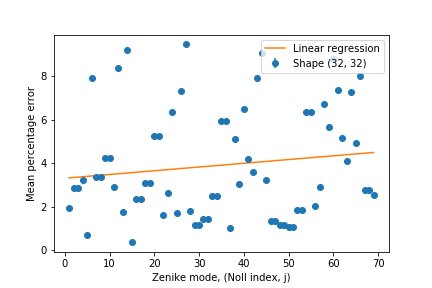
\includegraphics[width=\linewidth]{images/Zernike_fitting_percentage_error_one_mode_32_shape.png}
		\caption{}
		\label{fig:Zernike_fitting_percentage_error_one_mode_32_shape}
	\end{subfigure}
	\begin{subfigure}{0.48\textwidth}
		\centering
		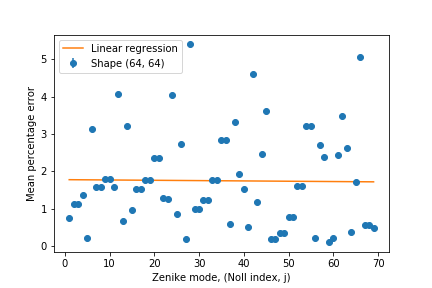
\includegraphics[width=\linewidth]{images/Zernike_fitting_percentage_error_one_mode_64_shape.png}
		\caption{}
		\label{fig:Zernike_fitting_percentage_error_one_mode_64_shape}
	\end{subfigure}
	
	\begin{subfigure}{0.48\textwidth}
		\centering
		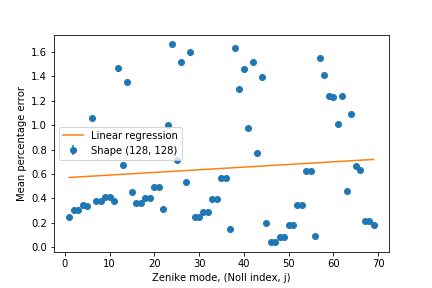
\includegraphics[width=\linewidth]{images/Zernike_fitting_percentage_error_one_mode_128_shape.png}
		\caption{}
		\label{fig:Zernike_fitting_percentage_error_one_mode_128_shape}
	\end{subfigure}
	\begin{subfigure}{0.48\textwidth}
		\centering
		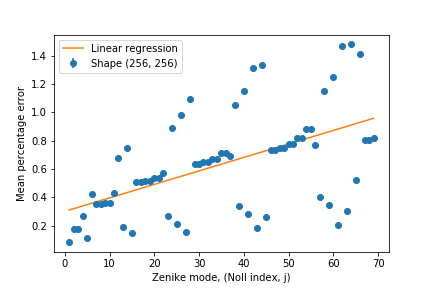
\includegraphics[width=\linewidth]{images/Zernike_fitting_percentage_error_one_mode_256_shape.png}
		\caption{}
		\label{fig:Zernike_fitting_percentage_error_one_mode_256_shape}
	\end{subfigure}
	\caption[The effect of image size on Zernike mode fitting accuracy]{The 
		effect of image size on Zernike mode fitting accuracy. Each 
		subfigure shows the percentage error in the Zernike mode 
		measurement and the linear regression of all Zernike mode 
		measurements for images of size \textbf{(a)} $32\times32$ pixels 
		\textbf{(b)} $64\times64$ pixels \textbf{(c)} $128\times128$ pixels 
		\textbf{(d)} $256\times256$ pixels}
	\label{fig:zernike_fitting_accuracy}
\end{figure}

A wavefront may be dominated by a single Zernike mode, but they are almost 
never composed entirely of one Zernike mode. 
Figure~\ref{fig:Zernike_fitting_percentage_error_random_modes_repeat_resize_factor_1} shows the mean percentage error in the Zernike mode amplitude 
measurement for 50 wavefront, $256\times256$ pixel size, generated with 
random amplitudes for all 69 Zernike modes. Clearly, having multiple modes 
present simultaneously adds a degree of variance to the amplitude 
measurement accuracy as well as an overall increase in the error magnitude.

It is a time-consuming process for AOtools to generate wavefront images of 
sizes greater than $256\times256$ pixels, typically about a $0.1-1$ seconds 
per image depending on the overall size and number of Zernike modes 
simulated. In order to increase the speed of fitting, acquired wavefront 
images are often resized. This too has an effect on Zernike mode accuracy 
fitting since the resizing function bins multiple pixels together and takes 
their mean, effectively smoothing the wavefront. 
Figures~\ref{fig:Zernike_fitting_percentage_error_random_modes_repeat_resize_factor_2}-\ref{fig:Zernike_fitting_percentage_error_random_modes_repeat_resize_factor_8} show the same set of wavefronts used for the results in 
Figure~\ref{fig:Zernike_fitting_percentage_error_random_modes_repeat_resize_factor_1}, except that the wavefronts were resized by varying factors prior to the Zernike modes amplitude measurements. Clearly, the resizing factor is inversely proportional to the overall Zernike mode fitting accuracy.

\begin{figure}[h]
	\centering
	\begin{subfigure}{0.48\textwidth}
		\centering
		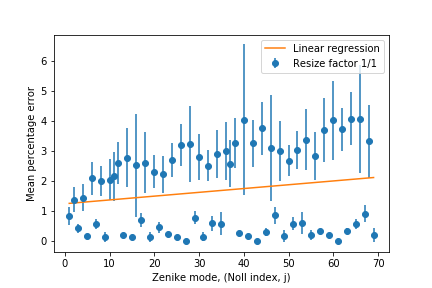
\includegraphics[width=\linewidth]{images/Zernike_fitting_percentage_error_random_modes_repeat_resize_factor_1.png}
		\caption{}
		\label{fig:Zernike_fitting_percentage_error_random_modes_repeat_resize_factor_1}
	\end{subfigure}
	\begin{subfigure}{0.48\textwidth}
		\centering
		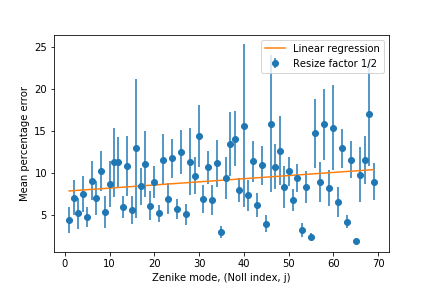
\includegraphics[width=\linewidth]{images/Zernike_fitting_percentage_error_random_modes_repeat_resize_factor_2.png}
		\caption{}
		\label{fig:Zernike_fitting_percentage_error_random_modes_repeat_resize_factor_2}
	\end{subfigure}
	
	\begin{subfigure}{0.48\textwidth}
		\centering
		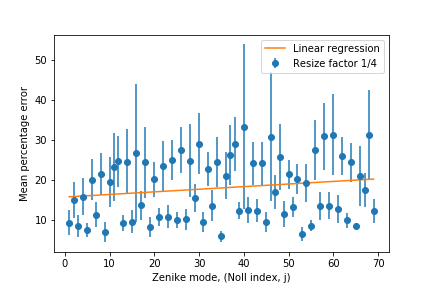
\includegraphics[width=\linewidth]{images/Zernike_fitting_percentage_error_random_modes_repeat_resize_factor_4.png}
		\caption{}
		\label{fig:Zernike_fitting_percentage_error_random_modes_repeat_resize_factor_4}
	\end{subfigure}
	\begin{subfigure}{0.48\textwidth}
		\centering
		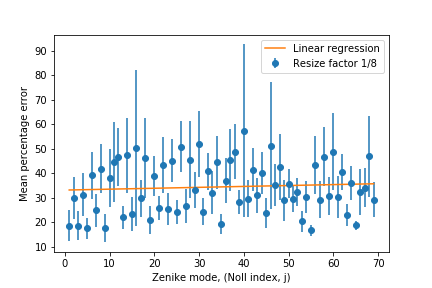
\includegraphics[width=\linewidth]{images/Zernike_fitting_percentage_error_random_modes_repeat_resize_factor_8.png}
		\caption{}
		\label{fig:Zernike_fitting_percentage_error_random_modes_repeat_resize_factor_8}
	\end{subfigure}
	\caption[The effect of image resizing on Zernike mode fitting 
	accuracy]{The effect of image resizing on Zernike mode fitting 
		accuracy. An original image of size $256\times256$ pixels was 
		generated. Each subfigure shows the percentage error in the Zernike 
		mode measurement and the linear regression of all Zernike mode 
		measurements for images resized by \textbf{(a)} $1$ i.e. no 
		resizing \textbf{(b)} $\frac{1}{2}$ i.e $128\times128$ pixels 
		\textbf{(c)} $\frac{1}{4}$ i.e $64\times64$ pixels \textbf{(d)} 
		$\frac{1}{8}$ i.e. $32\times32$ pixels}
	\label{fig:zernike_fitting_accuracy_resize}
\end{figure}

There accuracy of the Zernike mode amplitude fitting is a limiting factor in two key areas. Firstly, the accuracy of the Zernike mode fitting is one of the limiting factors to acquiring an ideal control matrix and, therefore, the ideal characterisation assay shown in Figure~\ref{fig:characterisation_assay_ideal}. Secondly, the accuracy of the Zernike mode fitting is one of the limiting factors to acquiring a perfectly flat wavefront through direct wavefront sensing.

\subsection{Sensorless correction accuracy}
\label{subsec:sensorless_accuracy}

In order to make sensorless correction accessible to users the entire 
workflow detailed in Section~\ref{subsec:sensorless_correction} is 
automated. The image quality metric is measured for each image and Python's 
\textit{scipy}'s \textit{curve\textunderscore fit} 
functionality\cite{virtanen2020scipy} is used to fit a Gaussian function of 
the form:

\begin{equation}\label{eq:gaussian}
f(x) = (\Delta - \eta) + \eta e^{-\frac{\left(x-\mu\right)^{2}}{2\sigma^{2}}},
\end{equation}

to the data, where $\Delta$ is the offset value, $\eta$ is the 
normalisation constant, $\mu$ is the mean, and $\sigma$ is the standard 
deviation. The Zernike mode amplitudes applied and the image quality metric 
measurements are used as the $x$ and $f(x)$ variables respectively. 
\textit{scipy}'s \textit{curve\textunderscore fit} functionality then 
estimates the values of $\Delta$, $\eta$, $\mu$, and $\sigma$ which give 
the best fit to the data. An amplitude $\mu$ of the current Zernike mode is 
then applied to obtain the optimum correction for that mode. It is wise to 
constrain the values which these parameters can take, otherwise it is 
possible for the automation to go awry.

Figure~\ref{fig:zernike_fitting_only_current_power_metric_no_fit_2} shows 
some sample image quality metric values acquired from a correction routine 
on a \textit{Drosophila} neuro-muscular junction preparation similar to 
that shown in Section~\ref{sec:DeepSIM_biology}. Here the metric 
measurements were acquired for Zernike mode 5 (Noll index) using the 
Fourier Power metric from Section~\ref{subsec:fourier_power_metric} and the 
sampled Zernike mode amplitudes were $[-2,2]$ radians. If \textit{scipy}'s 
\textit{curve\textunderscore fit} functionality is applied with no 
constraints, the fitting shown in 
Figure~\ref{fig:zernike_fitting_current_power_metric_no_bound_2} is 
obtained. Clearly, there are two problems with this fit. Firstly, the value 
of $\mu$ is $-688$ radians - a frankly absurdly high aberration, certainly 
not physically possible for the sample type and depth of imaging in 
question, and not an aberration amplitude the ALPAO-69 DM on DeepSIM is 
capable of applying. Secondly, the fit has allegedly found a minimum as 
opposed to the desired maximum image quality for this mode. 

Imposing the boundary condition that $\mu \in [z_{l}, z_{u}]$ yields 
Figure~\ref{fig:zernike_fitting_current_power_metric_range_bound_2}. Here 
$z_{l} = z_{min} - 0.25(z_{max}-z_{min})$ and $z_{u} = z_{max} + 
0.25(z_{max}-z_{min})$ where $z_{max}$ and $z_{min}$ are the maximum and 
minimum Zernike mode amplitudes applied. The amplitude acquired is of a 
sensible order of magnitude, $1.85$ radians, however the fit still acquires 
a minimum. Imposing the boundary condition that $\eta \in [0, \infty)$ 
yields Figure~\ref{fig:zernike_fitting_current_power_metric_bound_2}. These 
boundary conditions guarantee that the value of $\mu$ is both of a sensible 
order of magnitude and corresponds to a maximum. It is worth noting that 
the image quality amplitude for data points corresponding to ``Zernike 
amplitude for maximum quality'' in 
Figure~\ref{fig:sensorless_fitting_accuracy} do not represent the true 
image quality metric measurement when that amplitude is applied, only the 
theoretical image quality metric value according to the obtained fit. 

\begin{figure}[h]
	\centering
	\begin{subfigure}{0.48\textwidth}
		\centering
		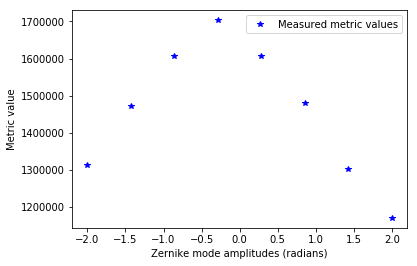
\includegraphics[width=\linewidth]{images/zernike_fitting_only_current_power_metric_no_fit_2.png}
		\caption{}
		\label{fig:zernike_fitting_only_current_power_metric_no_fit_2}
	\end{subfigure}
	\begin{subfigure}{0.48\textwidth}
		\centering
		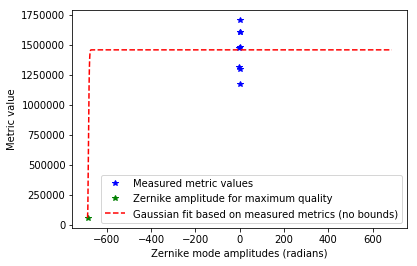
\includegraphics[width=\linewidth]{images/zernike_fitting_current_power_metric_no_bound_2.png}
		\caption{}
		\label{fig:zernike_fitting_current_power_metric_no_bound_2}
	\end{subfigure}
	
	\begin{subfigure}{0.48\textwidth}
		\centering
		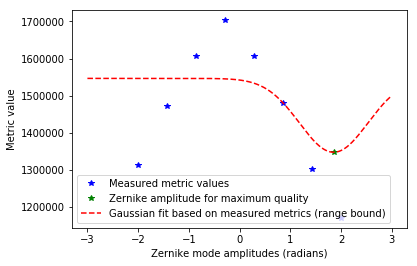
\includegraphics[width=\linewidth]{images/zernike_fitting_current_power_metric_range_bound_2.png}
		\caption{}
		\label{fig:zernike_fitting_current_power_metric_range_bound_2}
	\end{subfigure}
	\begin{subfigure}{0.48\textwidth}
		\centering
		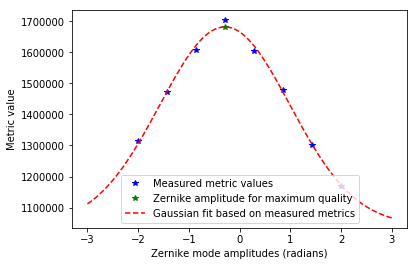
\includegraphics[width=\linewidth]{images/zernike_fitting_current_power_metric_bound_2.png}
		\caption{}
		\label{fig:zernike_fitting_current_power_metric_bound_2}
	\end{subfigure}
	\caption[Effect of parameter bounds on sensorless correction fitting accuracy]{Effect of parameter bounds on sensorless correction fitting accuracy. Metric measurements were acquired for Zernike mode 5 (Noll index) using the Fourier Power metric from Section~\ref{subsec:fourier_power_metric} \textbf{(a)} Measured metric values \textbf{(b)} Gaussian fit with no parameter bounds \textbf{(c)} Gaussian fit with bound on $\mu$ \textbf{(c)} Gaussian fit with bound on $\mu$ and $\eta$}
	\label{fig:sensorless_fitting_accuracy}
\end{figure}

Of course, these boundary conditions do not guarantee a good fit to the data, but they do eliminate some sources of fitting error. If the sample aberration is primarily from one source - i.e. spherical aberration mismatch - then correcting for aberration modes with smaller amplitudes can prove challenging since the image quality is already heavily degraded. Similarly, if the fit for one mode is poor and leads to an incorrect Zernike mode amplitude being applied, this can bias future image quality measurements and prevent correction of subsequent Zernike modes. The first case explains why the order Zernike modes are corrected in, specified by the user in the interface shown in Figure~\ref{fig:DM_sensorless_ao_parameters}, is important. The second case explains the existence of the "Reset DM" and "Apply last pattern" buttons in Figure~\ref{fig:DM_methods_cockpit}. "Reset DM" returns all actuators to their default 0 position. "Apply last pattern" applies the last recorded actuator pattern applied to the DM. Actuator patterns applied through "Reset DM" are not recorded. These buttons allow a user to toggle between the calculated sensorless correction pattern and no correction pattern. For a successful sensorless correction pattern, the improvement in image quality will be visually apparent. For a sensorless correction where an incorrect correction for one mode has caused a run-away degradation of the image quality, this too will be visually apparent.

\section{Future development}
\label{sec:future_dev}

Chapter~\ref{chpt:ao_tools} discussed the specific methods implemented in 
Microscope-AOtools for both AO device set up and operation. These Set-up 
and  Sample Correction methods rely on suites of techniques, wavefront 
sensing and image quality metric assessment respectively. These are 
designed to be easily extensible by users as new techniques are developed. 
The functions defining the existing wavefront sensing and image quality 
metric assessment techniques are stored in separate files. Which wavefront 
sensing technique will be used is an attribute of the highest level
of the code hierarchy and is used to select a wavefront sensing technique 
from the unwrapping method dictionary. Similarly, which image quality 
metric assessment will be used is an attribute of a lower level	of the 
code hierarchy and is used to select a wavefront sensing technique from 
the dictionary of image quality metrics. A detailed guide of where the 
appropriate classes and dictionaries are located and how to add new 
wavefront sensing and image quality metric assessment techniques is 
included in the \textit{README.md} file for Microscope-AOtools. Briefly, 
these suites are composed of functions with a defined set of input and 
output variables. A user creates a new wavefront sensing or image 
quality metric assessment functions with the input and outputs defined 
in the \textit{README.md}, adds this function to the correct file and 
then adds the function option to the correct suite dictionary.

Microscope-AOtools has been designed so a user can take an adaptive element 
in an arbitrary set-up, calibrate the adaptive element and use it on any 
sample type in a range of imaging modalities. Since Microscope-AOtools 
leverages Python-Microscope it already supports a number of adaptive 
elements, mostly deformable mirrors, which will expand as hardware support 
in Python-Microscope expands. Adding new devices to Python-Microscope is 
relatively simple. Refer to Python-Microscope 
(\url{https://www.python-microscope.org/}) for more details. 
Microscope-AOtools only requires that the adaptive element be a 
Python-Microscope device which has an attribute \textit{n\textunderscore 
	actuators} which defines the number of variable components of the device.

The process of setting up an adaptive element requires a wavefront sensor 
to observe the shape of the phase wavefront and calibrate how the variable 
components of the adaptive element affect this wavefront. By designing the 
set-up methods in Microscope-AOtools to accept any method from a suite of 
wavefront sensing techniques, Microscope-AOtools is both generalised and 
easily extensible. If the desired wavefront sensing technique is not 
already incorporated then a user only has to add the function necessary to 
perform the wavefront sensing step rather than to reimplement the set-up 
methods in their entirety. Swapping between wavefront sensing techniques is 
not implemented in the Cockpit user interface (UI) for AO control since the 
sensing technique is generally reliant on the physical setup and is 
unlikely to change between experiments.

Microscope-AOtools is further generalised as it allows for the control 
matrix to be acquired by some external method and then set in 
Microscope-AOtools with the \textit{set\textunderscore controlMatrix} 
method. This ensures that a user with an existing calibration routine 
wishing to access the sensorless AO methods in Microscope-AOtools can do so 
without having to repeat work they have already performed. It also allows 
control matrices acquired from routines using different phase acquisition 
techniques to be compared. Characterisation assays can be acquired for each 
method's control matrix and the accuracy of the Zernike mode recreation 
compared.

The generalised nature of Microscope-AOtools continues into the Sample 
Correction methods. By allowing the user to swap between wavefront sensing 
technique, Microscope-AOtools already possesses all the methods necessary 
for performing sample correction using direct wavefront sensing, provided 
the wavefront sensing technique is already included in the suite of 
methods. Similarly, Microscope-AOtools utilises a suite of image quality 
metrics suited to different sample types and imaging modalities. A user can 
select a pre-existing metric well suited to their application. If no 
appropriate metric currently exists a new one can easily be implemented 
and added  to the suite of metrics. Once implemented it can be used in any 
of the sensorless AO analysis methods outlined in 
Figure~\ref{fig:sensorless_correction_method}. Since the best image quality 
metric can vary between samples, this variable is left configurable from 
the Cockpit UI as shown in Figure~\ref{fig:DM_methods_cockpit_options}. A 
user need only add the appropriate label for the newly implemented image 
quality metric assessment technique to the options present in the Cockpit 
device code and it will be available with the other techniques shown in 
Figure~\ref{fig:DM_methods_cockpit_options}.

Furthermore, Microscope-AOtools allows for Zernike mode amplitudes to be 
set directly with the \textit{set\textunderscore phase} method. This means 
that if a user has an offline analysis technique, such as a machine 
learning approach, Microscope-AOtools can be used to calibrate the 
deformable mirror, the sample induced calculations are performed offline 
and then the appropriate correction applied through Microscope-AOtools.

Microscope-AOtools is free and open-source. It is intended to be a resource 
for the microscopy community at large and it is designed to minimise the 
time and effort spent replicating work other AO users have already done. As 
Microscope-AOtools acquires a larger base of users, some adding their own 
wavefront sensing techniques or image quality metrics to expand the 
existing suites, future and existing users will have a wider array of 
usability options, accelerating the adoption of novel techniques by the 
microscopy community and lowering the barrier to entry to set-up an AO 
system.

Beyond the open-ended task of expanding the existing suite of phase 
acquisition techniques and image quality metrics, there are a number of 
future developments that could be made to Microscope-AOtools. There does 
not currently exist a universal image quality metric, although strides have 
been made in that direction\cite{antonello2020multi}. Image quality metrics 
attempt to assign a numerical value for how `good' an image is, but what 
makes a `good' image varies between imaging modalities, sample type and 
even users. Most metrics pick some aspect of the image deemed to be 
significant (e.g. contrast, sharpness, maximum intensity, etc) and maximise 
it. Since Microscope-AOtools has access to multiple image quality metrics, 
one development would be designing a sensorless AO routine which measures 
multiple image qualities simultaneously, assigns some weight to each metric 
measurement and maximises the image quality based on several criteria.

Another direction for further development concerns restructuring the 
sensorless correction workflow. As explained in 
Section~\ref{subsec:sensorless_correction}, each Zernike mode is corrected 
for separately. There is an underlying assumption here that since the 
Zernike modes themselves are an orthonormal basis set, the effect they have 
on the image quality must also be orthogonal. However, phenomena such as 
the focal shift which accompanies spherical aberration would suggest that 
this is not necessarily the case\cite{torok1997role}. It may therefore be 
possible to obtain the optimum image quality faster and with fewer images 
with the kind of solvers used objective function maximisation, such as the 
Nelder-Mead method, than the current uni-variant 
approach\cite{nelder1965simplex}. Such an approach has been shown to work 
in principle on point objects to recover diffraction limited images but has 
not yet been demonstrated on biological samples\cite{murray2005wavefront}.

Finally, the integration of adaptive optical elements, primarily deformable 
mirrors, into Cockpit allows for the construction of remote focusing 
experiments. In remote focusing experiments, the adaptive element is used 
to shift the focal plane by applying a known amount of optical aberrations 
to the beam path, instead of manually moving the sample plane. This allows 
for higher axial scan speeds - since deformable mirrors are, on average, an 
order of magnitude faster than mechanical stages - and avoids mechanical 
interference between the objective lens and the sample through dipping 
media such as water or oil\cite{botcherby2008optical,vzurauskas2017rapid} 
This would require constructing another calibration routine to obtain the 
maps between physical displacement and defocus aberration applied in order 
to ensure accurate and reliable remote focusing.
